\documentclass[spanish]{udpreport}
\usepackage[utf8]{inputenc}
\usepackage[spanish]{babel}
\usepackage{enumerate}
\usepackage[]{float}

\title{Comprobación del funcionamiento del algoritmo STP e implementación de VLAN}

\author{Javiera Araya,
       Benjamin Morales,
        Fabian Estefania,
        Nicolas Pino.\\
        Profesor:Jaime Álvarez.\\
        Ayudante:Maximiliano Vega.} 

\begin{document}
\maketitle




\chapter*{Resumen} 
\addcontentsline{toc}{section}{Resumen} 
\markboth{RESUMEN}{RESUMEN} 




En la presente experiencia de laboratorio se estudia el comportamiento de la implementación del protocolo STP en una red LAN, por otro lado e igualmente parte de la experiencia de laboratorio, se realiza implementaciones de VLAN, las cuales se configuran acorde a los requerimientos personales a los cuales se quiera enfocar, junto con lo anterior mencionado se estudia asimismo su funcionamiento al momento de implementar la VLAN.

Finalmente, todos estos análisis anteriormente mencionados se logran con el programa de simulación de redes Cisco Packet Tracer.

\tableofcontents

\chapter{Introducción}
La presente experiencia de laboratorio se enfocara en el estudio y comprensión del protocolo STP y la implementación de una VLAN en una red, pero fuera de los aspectos generales para los que se pondrá en práctica esta experiencia hay que destacar a que se refiere el protocolo STP e igualmente señalar que tan importante es realizar configuración VLAN en una red.\\

STP es un protocolo de capa 2 del modelo OSI, trabaja con Switch y Bridges, su principal función es evitar la presencia de bucles en una topología con enlaces redundantes, para ello este protocolo actúa de manera tal que permite la activación y desactivación de enlaces de conexión. El estándar de STP es IEEE 802.1D.\\

Por otra parte VLAN es un método para crear redes lógicas dentro de una misma topología física, así actúan de manera independiente dentro de una misma red. Las ventajas de la implementación de VLAN son muchas pero una de las más importantes es la división de los grandes dominios broadcast en unos mas pequeños, así se limita la cantidad de dispositivos que participen en una tormenta broadcast. Otro de los beneficios de usar VLAN es la viabilidad para administrar la red, en otras palabras el administrador se encarga de colocar las políticas de acceso y seguridad para los grupos de usuario que genere a partir de VLAN.

\chapter{Desarrollo}

\section{Actividad I}
En esta actividad creamos una red compuesta por tres switches y 3PCs sin realizar ninguna de las configuraciones de STP.

\begin{figure}[H]
\begin{center}
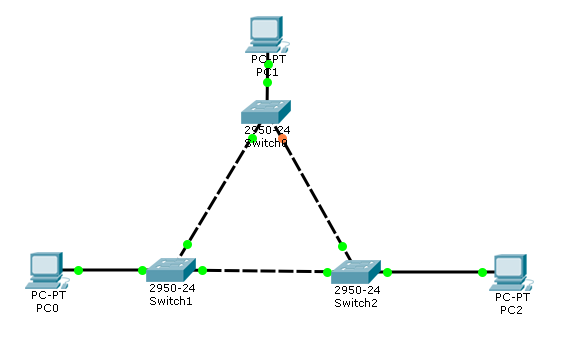
\includegraphics[scale=0.7]{images/sinSTP.PNG}
\end{center}
\end{figure}
\subsection{ ¿Qué camino realizara un paquete que para llegar desde el switch 0 hasta el switch2?}
El frame fue enviado a traves del PC1, automaticamente el puerto entre el switch 0 y el switch 2 se cerro, luego de que el frame accedio al switch 0, siguio la ruta accediendo al switch 1 para luego ingresar al switch 2 \\\\
Ruta seguida por el frame:PC0-SW0-SW1-SW2-PC2.

\subsection{ ¿Qué camino realizara un paquete que para llegar desde el switch 2 hasta el switch1?}
Como la configuracion entre puertos de los switches no cambio desde el caso anterior, el frame que fue enviado desde el PC2 paso de forma directa desde el switch2 al switch1\\\\
Ruta seguida por el frame:PC2-SW2-SW1-PC0.

\section{Actividad II}
En esta actividad se creo una red en donde se configuraron los protodolos STP en los Switches a travez de consola de cada switch\\
Definimos el switch 2 como root utilizando los siguientes comandos:\\
Switch Enable\\
Switch configure terminal\\
Switch(config)spanning-tree vlan 1 root primary\\\\

Luego definimos el switch 1 y el switch 0 como secundarios utilizando los siguientes comandos en cada uno de los switch.\\
Switch Enable\\
Switch configure terminal\\
Switch(config)spanning-tree vlan 1 root  secondary\\\\

\begin{figure}[H]
\begin{center}
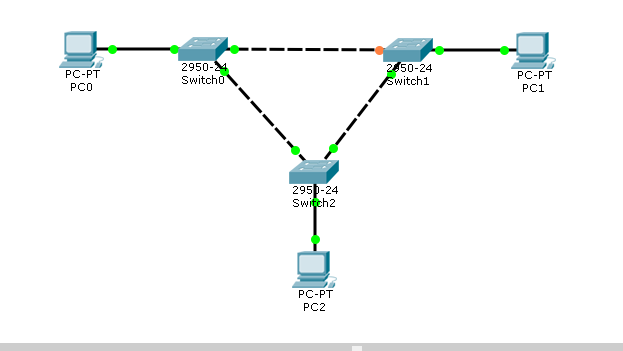
\includegraphics[scale=0.7]{images/conSTP.PNG}
\end{center}
\end{figure}

Luego de aplicar las configuraciones los puertos entre el switch 0 y el switch 1 se bloquean ya que son los switches secundarios, esto se hace para no producir bucles dentro de la red.

\subsection{¿Qué camino realizara un paquete que para llegar desde el switch 2 hasta el switch0?}
Se envia un mensaje desde el PC2 al PC0, como el switch 2 es el switch primario o root, el mensaje pasa directamente del switch 2 al switch0, luego el mensaje llega a su destino pasando del switch0 al PC0.\\\\
Ruta seguida por el frame:PC2-SW2-SW0-PC0.

\subsection{¿Qué camino realizara un paquete que para llegar desde el switch 1 hasta el switch0?}
Como el puerto entre el switch 1 y el switch 0 esta cerrado por la configuracion STP para evitar bucles, si se envia un mensaje desde el PC1 al PC0, el frame debe pasar obligatoriamente por el switch2 para poder acceder al switch 0 y al PC0, por lo que la ruta seguida por el frame es: PC1-SW1-SW2-SW0-PC0

\section{Actividad III: PRIORIZACIÓN EN STP}
En esta actividad se configuro la prioridad en cada uno de los switches con los siguientes comandos\\
Switch Enable\\
Switch configure terminal\\
Switch(config) spanning-tree vlan 1 priority "priority number"\\

en donde "priority number" es el numero de la prioridad que tendra el switch, mientras mas bajo, mayor prioridad tendra.\\\\

En nuestro caso lo configuramos de la siguiente forma:\\
Switch2=prioridad 1\\
switch1=prioridad 2\\
switch0=prioridad 2\\


\section{Actividad IV}
En esta Actividad se realizo la siguiente red configurando los enlaces entre switches en modo Trunk, ademas de agregar las Vlan (Vlan1, Vlan2, Vlan3, Vlan4)
y confirar los switches para asignar los PCs a sus Vlan correspondientes.\\\\
Vlan1=PC0 y PC7\\
Vlan2=PC1 y PC5\\
Vlan3=PC3 y PC6\\
Vlan4=PC2 y PC4\\
\begin{figure}[H]
\begin{center}
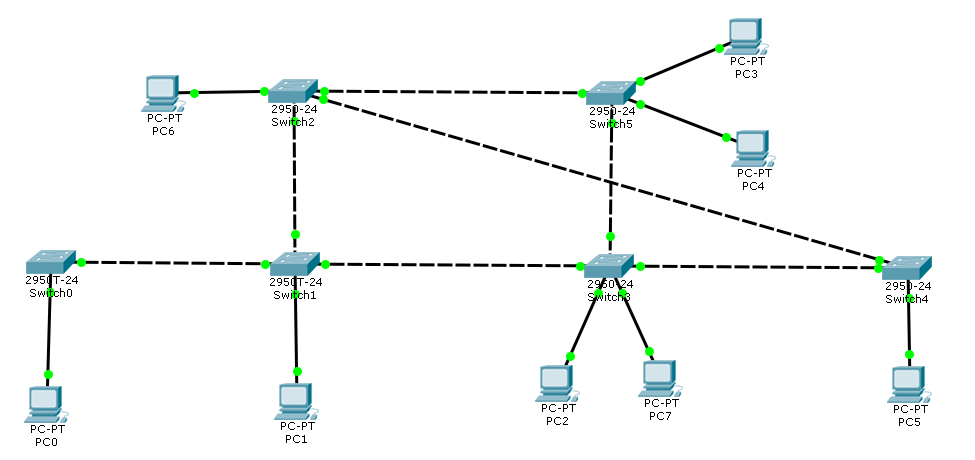
\includegraphics[scale=0.65]{images/VLAN.PNG}
\end{center}
\end{figure}

\subsection{¿Cuál es la diferencia del modo Access y el modo Trunk en un switch?}
La diferencia es que el modo Access solamente permite el paso de una única VLAN, en cambio el modo Trunk permite el paso de multiples VLAN a traves de el.\\

\subsection{¿Qué ocurre si conecto una puerta en modo Trunk a un PC?}
El PC quedara sin una Vlan especifica, por lo que el PC quedara asignado automaticamente a la Vlan por defecto (Vlan1) por el switch, por lo que este PC solo podra enviar y recibir mensajes de los equipos que pertenescan a la Vlan1.

\subsection{¿Qué ocurre si conecto dos switches, uno en modo access y otro en modo trunk?}
Ocurrira que solo se podra transmitir una VLAN a traves del enlace entre ambos switches, Esta  sera la VLAN permitida por el switch que esta en modo access, esto ocurrira en el caso donde los frames no tengan otra ruta que seguir.\\

\subsection{¿Qué camino realizara un paquete que para llegar desde el switch 1 hasta el switch 0?}
Extisten dos casos de como podria "reaccionar" el switch 0\\
1) Si se envia un mensaje desde un PC que tiene la misma VLAN que el PC que esta conectado al switch 0, entonces, el frame pasara del switch 1 al switch 0 y luego el frame pasara del switch 0 al PC0, un ejemplo de esto seria un mensaje enviado desde el PC7 al PC0, en el cual la ruta que seguiria el mensaje seria:\\PC7-SW3-SW1-SW0-PC0\\

2) Si se envia un mensaje desde un PC que no tiene la misma VLAN que el PC que esta conectado al switch 0, entonces, el frame pasara del switch 1 al switch 0 y luego el frame llegara solo hasta el switch 0 ya que la VLAN del mensaje no corresponde a la VLAN del PC que esta conectado al switch 0, un ejemplo de esto seria un mensaje enviado desde el PC1 al PC0, el cual la ruta que seguiria el mensaje seria:\\PC1-SW1-SW0.
\chapter{Conclusión}

A partir de lo realizado en la presente experiencia de laboratorio, se logra destacar varios puntos los cuales fueron fundamentales para el desarrollo de los objetivos propuestos, dichos puntos se especificaran a continuación.\\

La primera actividad se desarrolla en tres partes, esto es para ver en tiempo real lo que sucede con los cambios que se van realizando  en cada una de los procesos aplicados, los resultados obtenidos en cada parte del procedimiento cumplen fielmente con lo propuesto en los objetivos, vale decir que al momento de simular una red a base de bucles en Packet Tracer se analiza cada caso, se inicia sin realizar ningún tipo de configuración STP, posteriormente se configura el protocolo STP dentro de la red sin asignar un root, en otras palabras los switches elegirán cual será el root mediante la comparación de ID. Finalmente para el último caso se asigna prioridad a un switch como root, para cada uno de los tres casos se observa en camino que sigue cada paquete y los cambios de ruta que hace al configurar este protocolo.\\

La segunda actividad se centró en la implementación de VLAN esto llevo a la configuración de cada switch en una red LAN y observar el comportamiento de esta red (ya configurada) al hacer envíos de paquetes desde distintos host. Los resultados fueron favorables para lo que se tenía como objetivo de esta segunda parte de la experiencia, en otras palabras  se logró implementar de manera exitosa una red con distintas VLAN, esto se hizo claramente notorio al momento de enviar paquetes desde un host que estaba en una VLAN distinta al de otro host, la cual tuvo como resultado la no acogida del ya mencionado paquete enviado.\\

Finalmente se concluye que de la experiencia de laboratorio que se cumplen con los objetivos de ambas actividades, en síntesis, se logra una amplia comprensión del funcionamiento del protocolo STP y su importancia para la prevención en la formación de bucles. Por otra y con respecto a la implementación de VLAN en una red se consigue interpretar su funcionamiento, también cabe destacar lo importante que es este tipo de implementación (valga la redundancia) ya que esto da muchas facilidades en lo que a administración de red se refiere, actualmente este tipo de redes con VLAN se ven en muchos lugares de trabajo y el instituciones las cuales se requiere tener un uso responsable de los accesos a la información.



\end{document}



